\subsection{SAT $\propto$ 3--SAT}
\begin{enumerate}[(a)]
\item \begin{description}
\item[Énoncé de SAT] : \\
\begin{tabular}{r l l}
Données : & $ \mathcal{V} = \lbrace v_1, v_2 \ldots v_n \rbrace $ & \emph{Ensemble de $n$ variables}\\
& $ \mathcal{C} = \lbrace c_1, c_2, c_3 \ldots c_m \rbrace $ & \emph{Ensemble de $m$ clauses}\\
où & $ c_i = ( l_{i1} \vee l_{i2} \vee \cdots \vee l_{ik} ) $ & \emph{Clauses de $k$ littéraux}\\
avec & $ l_{ij} = v$ ou $ \neg v $ & \emph{avec $v \in U$} \\
\end{tabular}

Problème : existe-il au moins une affectation des variables telle que chaque clause de $\mathcal{C}$ soit vrai.

\item [Énoncé de 3--SAT] : 

3--SAT est identique au problème SAT avec $k = 3$.\\
\begin{tabular}{r l}
Données : & $ \mathcal{V} = \lbrace v_1, v_2, v_3 \ldots v_n \rbrace $\\
& $ \mathcal{C} = \lbrace c_1, c_2, c_3 \ldots c_m \rbrace $\\
où & $ c_i = ( l_{i1} \vee l_{i2} \vee l_{i3} ) $\\
avec & $ l_{ij} = v$ ou $ \neg v$\\
\end{tabular}
\end{description}
\item La réduction du problème SAT peut être définit en montrant que chaque clause $c$ de $\mathcal{C}$ peut-être transformée en un ensemble de clauses $\mathcal{C'}$ tel que pour toute affectation rendant vrai l'ensemble des clauses de $\mathcal{C}$, nous pouvons trouver une affectation rendant vrai chaque clause de $\mathcal{C'}$. Chaque clause de $\mathcal{C'}$ devant être de taille exactement 3. La réciproque doit également être montrée.

Définissons les réductions :

\begin{description}
\item \mathversion{bold} $k = 1$ \mathversion{normal}

Soit $ci_1$ une clause de taille 1, nous avons $ci_1 = (l)$.
Ajoutons deux variables $v_1, v_2 \notin \mathcal{V}$ et transformons la clause $c$ en quatre clauses. Nous obtenons l'ensemble $\mathcal{C}_1 = \lbrace c_1, c_2, c_3, c_4 \rbrace$ avec :
\[ c_1 = ( l \vee v_1 \vee v_2 )\]
\[ c_2 = ( l \vee v_1 \vee \neg v_2 )\]
\[ c_3 = ( l \vee \neg v_1 \vee v_2 )\]
\[ c_4 = ( l \vee \neg v_1 \vee \neg v_2 )\]

\item \mathversion{bold} $k = 2$ \mathversion{normal}

Soit $ci_2$ une clause de taille 2, nous avons $ci_2 = ( l_1 \vee l_2 )$.
Ajoutons une variable $v \notin \mathcal{V}$ et transformons la clause $c$ en deux clauses. Nous obtenons l'ensemble $\mathcal{C}_2 = \lbrace c_1, c_2 \rbrace$ avec :
\[ c_1 = ( l_1 \vee l_2 \vee v )\]
\[ c_2 = ( l_1 \vee l_2 \vee \neg v )\]

\item \mathversion{bold} $k = 3$ \mathversion{normal}

La clause $ci_3$ ne subit pas de transformation.
\[ \mathcal{C}_3 = \lbrace ci_3 \rbrace \]

\item \mathversion{bold} $k > 3$ \mathversion{normal}

Soit la clause $ci_k = ( l_1 \vee l_2 \vee \cdots \vee l_k )$. Nous ajoutons $(k - 3)$ nouvelles variables $(v_1, v_2 \ldots v_{k-3})$.

\[ \mathcal{C}_k = \underbrace{(l_1 \vee l_2 \vee v_1)}_{c_1} \bigwedge_{i=1}^{k-4}\left[ \underbrace{(\neg v_i \vee l_{i+2} \vee v_{i+1})}_{c_{i+1}}\right]  \wedge \underbrace{(\neg v_{k-3} \vee l_{k-1} \vee l_{k})}_{c_{k-2}} \]

Montrons que SAT est vrai si et seulement si 3--SAT est vrai :

\begin{description}
 \item \textbf{SAT $\rightarrow$ 3--SAT}
 
 	\begin{itemize}
 		\item Soit une interprétation $I_1$ qui satisfasse la clause $ci_1$ :
 		 \[ val(I_1,ci_1) = val(I_1,l) = vrai\]
 		
 		Prenons une interprétation $I_1'$ avec $val(I_1,l) = val(I_1',l)$, peu importe les affectations de $v_1$ et $v_2$, $l$ étant présent dans toutes les clauses de $\mathcal{C}_1$ :
 		\[ val(I_1',\mathcal{C}) = \top \]
 		
 		\item Soit une interprétation $I_2$ qui satisfasse la clause $ci_2$ :
 		\[ \exists i, val(I_2,l_i) = \top \]
 		Prenons une interprétation $I_2'$ avec :
 		\[ val(I_2,l_1) = val(I_2',l_1) \]
  		\[ val(I_2,l_2) = val(I_2',l_2) \]
  		Peu importe l'affectation de $v$ dans $I_2'$, nous avons $val(I_2',\mathcal{C}_2) = \top$.
  		
  		\item Soit une interprétation $I_k$ qui satisfasse la clause $ci_k$ :
  		\[ \exists i, val(I_k,l_i) = \top \]
  		
  		Prenons une interprétation $I_k'$ telle que :
  		\begin{eqnarray*}
  		val(I_k,l_i) & = & val(I_k',l_i)  \\
  		\forall j \in \mathbb{N}^* \mid j \leq (i-2), val(I_k', v_j) & = & \top \\
  		\forall j \in \mathbb{N}^* \mid (i-1) \leq j \leq (k-3), val(I_k', v_j) & = & \bot \\
  		\end{eqnarray*}
  		
  		Nous obtenons :
  		\[ val(I_k',\mathcal{C}_k) = \top\]
  		
 	\end{itemize}
 	
 \item \textbf{3--SAT $\rightarrow$ SAT}
 
 	\begin{itemize}
 	\item Prenons une interprétation $I_1$ telle que $val(I_1,\mathcal{C}_1) = \top$.
 	
 	Sans perte de généralité, nous supposons que : 
 	\[ val(I_1,v_1) = val(I_1,v_2) = \top \]
 	La clause $c_4$ de $\mathcal{C}_1$ ne peut être satisfaite que si $val(I_1,l) = \top$.
 	
 	Nous avons donc :
 	\[ val(I_1,ci_1) = \top \]
 	
 	\item Prenons une interprétation $I_2$ telle que $val(I_2,\mathcal{C}_2) = \top$.
 	
 	Sans perte de généralité supposons que :
 	\[val(I_2,v) = \top \]
 	
 	La clause $c_2$ de $\mathcal{C}_2$ ne peut être satisfaire que si $val(I_2,(l_1 \vee l_2)) = \top$.
 	
 	Nous avons donc :
 	\[ val(I_2,ci_2) = \top \]
 	
 	\item Prenons une interprétation $I_k$ telle que $val(I_k,\mathcal{C}_k) = \top$ et montrons qu'il existe forcément un $i$ tel que $val(I_k,l_i) = \top$.
 	
 	Supposons que l'interprétation $I_k$ est modèle de $\mathcal{C}_k$ avec 
 	\[ \forall i \in \mathbb{N}^* \mid i \leq k, val(I_k,l_i) = \bot \]
	\[ \Rightarrow val(I_k,v_1) = \top  \textrm{ (dans $c_1$)} \]
	Donc :
	
	\begin{tabular}{lrl}
		& $\forall i \in \mathbb{N}^* \mid i \leq (k-4), val(I_k,v_{i+1})$ & $= \top$ \\
		$\Rightarrow$ & $val(I_k,v_{k-3})$ & $= \top$ \\
		$\Rightarrow$ & $val(I_k,c_{k-2})$ & $= \bot$ \\
		$\Rightarrow$ & $val(I_k,\mathcal{C}_k)$ & $= \bot$
	\end{tabular}
	
	Pour que l'interprétation $I_k$ satisfasse $\mathcal{C}_k$, il doit exister un $i \in \mathbb{N}^*$ tel que $i \leq k$ et que $val(I_k,l_i) = \top$.
	
	Nous avons donc :
	\[ val(I_k,ci_k) = \top \]
 	 	
 	\end{itemize}
 
\end{description}

\end{description}

\item Le point (b) définit la réduction de SAT vers 3--SAT. Afin de montrer la NP-Complétude de 3--SAT, montrons que la réduction s’effectue en un temps polynomial.

Soit :
\begin{description}
\item $k$ la taille de la clause initiale,
\item $v_k$ le nombre de variables à ajouter pour obtenir des clauses de taille 3,
\item $w_k$ le nombre de clauses de taille 3 obtenues à partir de la clause initiale.
\end{description}
\begin{center}
\begin{tabular}{c c}
$v_3 = 0$ & $w_3 = 1$ \\
$v_4 = 1$ & $w_4 = 2$ \\
$v_5 = 2$ & $w_5 = 3$ \\
\vdots & \vdots
\end{tabular}
\end{center}

Pour tout $k > 3$ :
\[ v_k = v_{\left \lceil \frac{k}{2} \right \rceil + 1} + v_{\left \lfloor \frac{k}{2} \right \rfloor + 1} + 1 \]
\[ w_k = w_{\left \lceil \frac{k}{2} \right \rceil + 1} + w_{\left \lfloor \frac{k}{2} \right \rfloor + 1} \]

$v_k = \theta(k)$, donc borné par la taille de F. La réduction s'effectue donc en un temps polynomial.

Il est possible de réduire le problème SAT à 3--SAT en un temps polynomial, SAT étant NP-complet, 3--SAT l'est aussi.
\item Soit $\mathcal{C}$ un ensemble de clause à $n_v$ variables avec $n_1$ clauses de taille 1, $n_2$ clauses de taille 2, $n_3$ clauses de taille 3, $n_4$ clauses de taille 4 et $n_5$ clauses de taille 5. Calculons le nombre de variables et le nombre de clauses obtenues après réduction (respectivement $n_v'$ et $n_c'$).

Les points (b) et (c) permettent de déterminer pour une clause de taille $k$, le nombre de clause obtenues et le nombre de variables ajoutées après réduction. Nous pouvons donc en déduire la tableau suivant :

\begin{tabularx}{\textwidth}{| X || c | c | c | c | c |}
\hline
Taille de la clause dans $\mathcal{C}$	& 1 	& 2 	& 3 	& 4 	& 5 	\\
\hline
Nombre de clauses						& $n_1$	& $n_2$	& $n_3$	& $n_4$	& $n_5$	\\
\hline
Nombre de variables ajoutées par clause	& 2		& 1 	& 0 	& 1 	& 2 	\\
\hline
\textbf{Nombre de variables ajoutées au total} 	& $2n_1$& $n_2$	& 0		& $n_4$	& $2n_5$\\
\hline
Nombre de clauses obtenues par clause 	& 4 	& 2 	& 1 	& 2 	& 3 	\\
\hline
\textbf{Nombre de clauses obtenues au total}	& $4n_1$& $2n_2$& $n_3$	& $2n_4$& $3n_5$\\
\hline

\end{tabularx}

Nous avons donc :
\[ n_v' = n_v + 2n_1 + n_2 + n_4 + 2n_5 \]
\[ n_c' = 4n_1 + 2n_2 + n_3 + 2n_4 + 3n_5 \]
\end{enumerate}

\subsection{3--SAT $\propto$ 2--SAT ?}
Cette réduction repose sur un principe qui consiste à décomposer une clause de taille $k$ en plusieurs clauses de tailles inférieures.

Soit une clause $c = (l_1 \vee l_2 \vee l_3)$ une clause de taille 3 et $I$ une interprétation qui satisfait $c$.

\begin{description}
\item[Cas 1 :] décomposons cette clause en deux clauses $c_1$ et $c_2$ de tailles 1 et 2 :
\begin{eqnarray*}
c_1&=&(l_1) \\
c_2&=&(l_2 \vee l_3)
\end{eqnarray*}
Pour montrer l'équivalence 3--SAT $\leftrightarrow$ 2--SAT, il faut ajouter une variable $v$ aux deux clauses créées :
\begin{eqnarray*}
c_1&=&(l_1 \vee v) \\
c_2&=&(l_2 \vee l_3 \vee \neg v)
\end{eqnarray*}

Nous avons donc la clause $c_2$ de taille 3.

\item[Cas 2 :] décomposons cette clause en trois clauses $c_1$, $c_2$ et $c_3$ de taille 1 :
\begin{eqnarray*}
c_1 & = & (l_1) \\
c_2 & = & (l_2) \\
c_3 & = & (l_3)
\end{eqnarray*}

Pour montrer l'équivalence 3--SAT $\leftrightarrow$ 2--SAT, il faut ajouter deux variables $v_1$ et $v_2$ aux trois clauses créées :
\begin{eqnarray*}
c_1 & = & (l_1 \vee v_1 \vee \neg v_2) \\
c_2 & = & (l_2 \vee \neg v_1 \vee v_2)\\
c_3 & = & (l_3 \vee v_1 \vee v_2)
\end{eqnarray*}
Nous avons donc également des clauses de taille 3. La réduction définie ci-avant ne permet donc pas la réduction de 3--SAT vers 2--SAT.
\end{description}

\subsection{2--SAT, un problème polynomial}
\begin{enumerate}[(a)]
\item Systèmes de deux clauses à deux littéraux :
\begin{description}
\item[Insatisfiable] : $(x \vee x) \wedge (\neg x \vee \neg x)$ \\
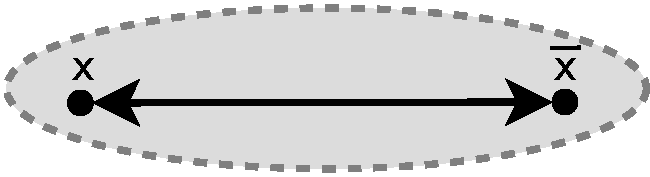
\includegraphics[width=5cm]{files/g1ex3.pdf}
\item[Valide] : $(x \vee \neg x) \wedge (\neg x \vee x)$ \\
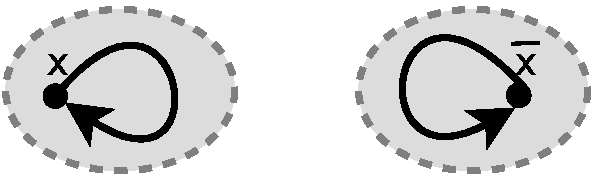
\includegraphics[width=5cm]{files/g2ex3.pdf}
\item[Contingent] : $(x \vee x) \wedge (x \vee x)$ \\
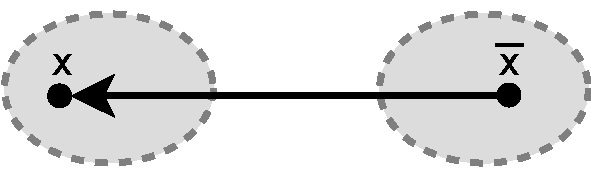
\includegraphics[width=5cm]{files/g3ex3.pdf}
\end{description}
\item 

Insaisissabilité du premier ensemble de clauses est clairement visible sur le graphe car les sommets $x$ et $\neg x$ sont dans la même composante fortement connexe.

Le deux autres ensembles sont satisfiables, les deux sommets ne sont pas dans la même composante fortement connexe.


\item L'algorithme suivant permet la génération du graphe correspondant à l'ensemble de clauses passé en paramètres, que nous appellerons graphe de satisfaction:

\begin{algorithm}[H]
  \caption{GrapheSatisfaction($\mathcal{C},\mathcal{V}$)}
  \Donnees{\\
  $\mathcal{C}$ \textit{// Ensemble de clauses}\\
  $\mathcal{V}$ \textit{// Ensemble des variables}
  }
  \Deb{
  Graphe.$\mathcal{S} = \emptyset$; \textit{// Ensemble des sommets du graphe}\\
  Graphe.$\mathcal{A} = \emptyset$; \textit{// Ensemble des arcs du graphe}\\
  \textit{// Initialisation des sommets}\\
  \PourTous{$v \in \mathcal{V}$}{
  ajouter(Graphe.$\mathcal{S}$,$v$)\;
  ajouter(Graphe.$\mathcal{S}$,$\neg v$)\;
  }
  \textit{// Parcours des clauses}\\
  \PourTous{$c \in \mathcal{C}$}{
  	ajouter(Graphe.$\mathcal{A}$,$(\neg c.x,c.y)$)\;
  	ajouter(Graphe.$\mathcal{A}$,$(\neg c.y,c.x)$)\;
  }
    \Retour Graphe\;
  }
\end{algorithm}
Cet algorithme effectue un parcours de $\mathcal{V}$ et un parcours de $\mathcal{C}$, sa complexité est donc $O(|\mathcal{C}|+|\mathcal{V}|)$.

\item Les composantes fortement connexes du graphe de satisfaction généré, ainsi que leur ordre topologique, peuvent être calculées par l'algorithme de Tarjan.

\begin{algorithm}[H]
  \caption{Tarjan\_Main($G$)}
  \Donnees{
  $G$ \textit{// Le graphe}
  }
  \Deb{
  date $\leftarrow 0$\;
  \PourTous{$s \in G.\mathcal{S}$}{
  DEBUT[$s$] $\leftarrow 0$\;
  CFC[$s$] $\leftarrow 0$\;
  }
  Pile $\leftarrow \emptyset$\;
  numCFC $\leftarrow 0$\;
  
  \PourTous{$s \in G.\mathcal{S}$}{
  \Si{DEBUT[$s$] $= 0$}{
  Tarjan\_Rec($s$,date,DEBUT,Pile,numCFC,CFC)\;
  }
  
  }
    \Retour Comp;
  }
\end{algorithm}

\begin{algorithm}[H]
  \caption{Tarjan\_Rec($s$,date,DEBUT,Pile,numCFC,CFC)}
  \Donnees{\\
  s \textit{// Le sommet}\\
  date \textit{// Date de visite du sommet courant}\\
  DEBUT \textit{// Tableau de dates de visites pour chaque sommet}\\
  Pile \textit{// Pile de sommets}\\
  numCFC \textit{// Numéro de la CFC}\\
  CFC \textit{// Liste des CFC}\\
  }
  \Deb{
	date $\leftarrow$ date$+1$\;
	DEBUT[$s$] $\leftarrow$ date\;
	min $\leftarrow$ DEBUT[$s$]\;
	Empiler(Pile,$s$)\;
	\PourTous{$v \in $Adj[$s$]}{
	\Si{DEBUT[$v$]$=0$}{
	min $\leftarrow$ MIN(min,Tarjan\_Rec($v$,date,DEBUT,Pile,numCFC,CFC)))\;
	}
	\SinonSi{CFC[$v$]$=0$}{
	min $\leftarrow$ MIN(min,DEBUT[$v$])\;
	}
	}
	\Si{min$=$DEBUT[$s$]}{
	Ncfc $\leftarrow$ numCFC $+1$\;
	}
	\Repeter{$k \neq s$}{
	$k \leftarrow$ Depiler(Pile)\;
	CFC[$k$] $\leftarrow$ numCFC\;
	}
    \Retour Comp;
	}
\end{algorithm}

L'algorithme \texttt{Tarjan\_Main} initialise la date de visite de chaque sommet à zéro. Nous constatons que les deux algorithmes exécutent \texttt{Tarjan\_Rec} uniquement sur des sommet dont la date de première visite est nulle. Or chaque appel à \texttt{Tarjan\_Rec} affecte une date de visite supérieure à zéro au sommet courant. \texttt{Tarjan\_Rec} est donc appelé exactement une fois par sommet.

De même, un sommet n'est empilé qu'à l'exécution de \texttt{Tarjan\_Rec}, donc chaque sommet ne sera empilé (et donc dépilé) qu'une seule fois. La boucle de l'algorithme \texttt{Tarjan\_Rec} (ligne 13) a une complexité globale en $O(|\mathcal{V}|)$.

En revanche, la bouche ligne 6 est effectuée une fois pour chaque voisin du sommet courant, donc $|\mathcal{V}|$ fois au pire pour chaque appelle. \texttt{Tarjan\_Rec} n'étant appelée que $|\mathcal{V}|$ fois en totale nous arrivons donc à une complexité de $O(|\mathcal{V}|^2)$.

Dans le pire des cas le nombre de variables d'une instance de 2--SAT est égale à deux fois le nombre de clauses (chaque clause comportant dans ce cas deux variables uniques). Or notre conversion génère deux sommets par variable. La complexité de l'algorithme en fonction du nombre de clauses est donc de $O(|\mathcal{C}|^2)$.

\item 
\begin{itemize}
\item Nous appellerons \emph{Absurd--Graph} le problème de décision consistant de savoir si une variable partage avec la négation une composante fortement connexe (ou $CFC$) du graphe de satisfaction. 
\item Tout arc ajouté par $GrapheSatisfaction$ correspond à une contrainte de la forme $((x \vee y) \wedge \neg x) \Rightarrow y)$, donc une implication. Étant donnée les $CFC$, calculés par l'algorithme de $Tarjan$, nous pouvons vérifier linéairement en le nombre de sommets si le graphe de satisfaction est \og absurde \fg, ce qui correspondrait effectivement à $(\neg(x) \Leftrightarrow x)$.
\item Dans le cas contraire il faut prendre l'inverse de l'ordre topologique calculée par $Tarjan$ et affecter les variables de chaque composante comme précise l'article de Philipe Gambette. Ceci nous garantie de ne pas avoir d'interprétations $( \bot \Rightarrow \top )$, seuls à pouvoir casser l'enchaînement des implications. 
\item Nous finissions alors soit avec une affection modèle, soit avec l'affirmation de l'insatisfiabilité de l'instance 2--SAT. Un algorithme pour résoudre \emph{Absurd--Graph} permet donc de résoudre le problème 2--SAT.
\end{itemize}
\end{enumerate}
